\documentclass[a4paper,12pt]{article}
\usepackage[utf8]{inputenc}

\usepackage[top=2cm,bottom=2cm,right=2cm,left=2cm]{geometry}
\usepackage{amsmath,amssymb,enumitem,multicol,graphicx,tikz,framed,tcolorbox,mathtools,comment,subcaption,array,pgfplots}
\usepackage{listings}
\usepackage{xcolor}
\linespread{1.3}
%New colors defined below
\definecolor{codegreen}{rgb}{0,0.6,0}
\definecolor{codegray}{rgb}{0.5,0.5,0.5}
\definecolor{codepurple}{rgb}{0.58,0,0.82}
\definecolor{backcolour}{rgb}{0.95,0.95,0.92}

%Code listing style named "mystyle"
\lstdefinestyle{mystyle}{
  backgroundcolor=\color{backcolour},   commentstyle=\color{codegreen},
  keywordstyle=\color{magenta},
  numberstyle=\tiny\color{codegray},
  stringstyle=\color{codepurple},
  basicstyle=\ttfamily\footnotesize,
  breakatwhitespace=false,         
  breaklines=true,                 
  captionpos=b,                    
  keepspaces=true,                 
  numbers=left,                    
  numbersep=5pt,                  
  showspaces=false,                
  showstringspaces=false,
  showtabs=false,                  
  tabsize=2
}

%"mystyle" code listing set
\lstset{style=mystyle}

\title{Code Listing}
\date{ }

\begin{document}
	DataBases
	\tableofcontents
	\newpage
	\section{What are they?}
	Databases are structured collections of data. The are used to store information. \\
	Databases are part of just about all aspects of business and digital technologies.\\
	Retail , banking,  social networks, any kind of reasonably sophisticated website, educational institutions , etc  all use them.\\
	Databases are made up of rows and columns of information and the simplest idea of a database is a table or spreadsheet.\\
	In order to store large amounts of information the data is organised into many different tables with connections (or relationships) between the tables.\\
	The data base must be designed so that information can be efficiently read , added, deleted.\\
	As databases often store personal data maintaining the integrity and security of data is essential.\\
	
	\section{What do we want to do with them?}
	We want to:
	\begin{itemize}
		\item Design the database so that it will efficiently hold information
		\item Put information in it
		\item Get information out of it
		\item Update information
		\item Delete information
		\item The above is sometimes acronymed to CRUD (Create Read Update Delete)
	\end{itemize}
Data bases can be created and managed using programming languages such as Python and PHP.\\
We will work directly to a data base using the SQLite Browser \\
The most common language used to manage a database is SQL (Structured Query Language)  (Which can be used in conjunction with the above languages).

	\section{Structure of a database table}
	\begin{figure}[!h]
		\centering
		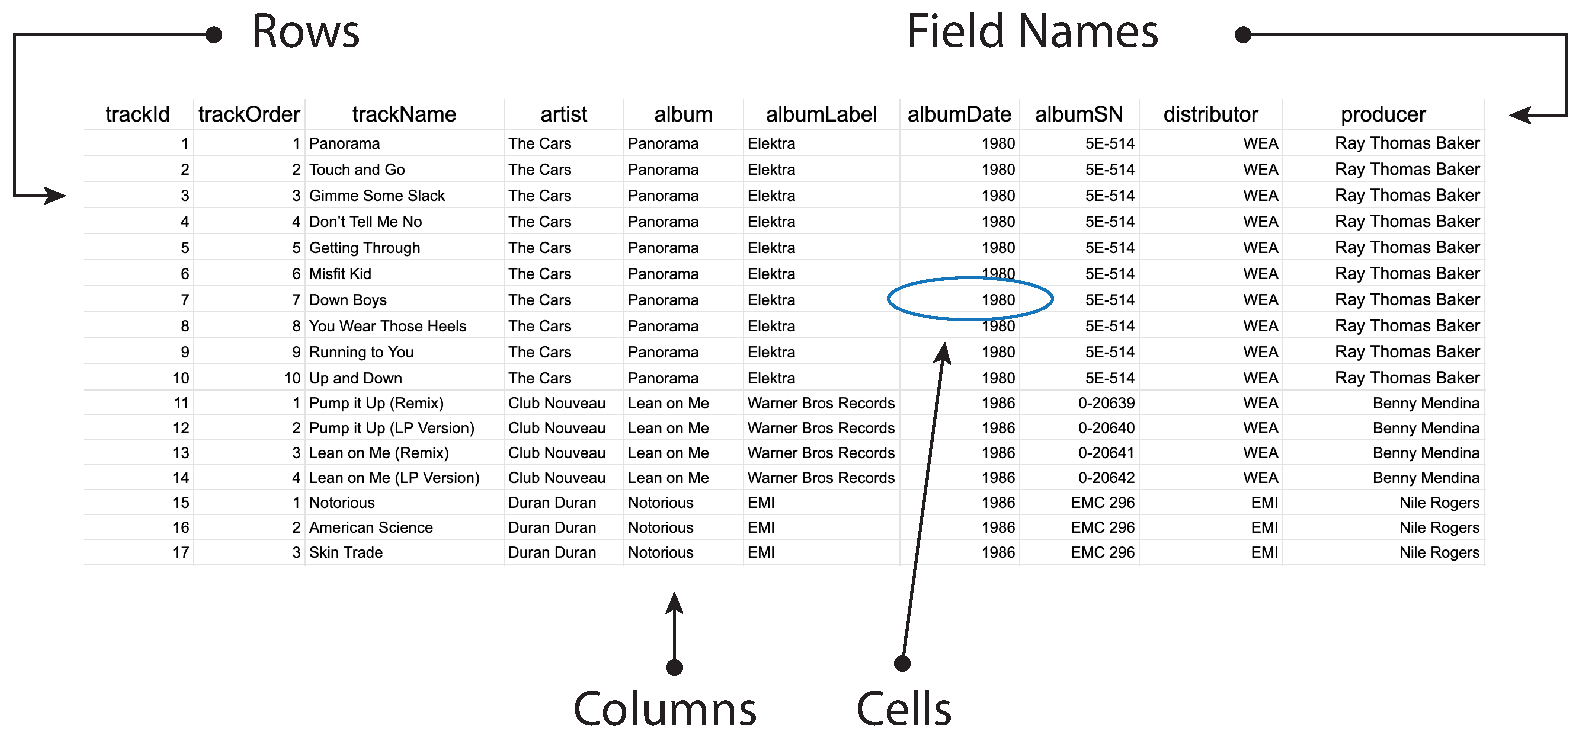
\includegraphics[width=16.5cm]{dBase_digram_copy.pdf}
	\end{figure}
\section{Designing: part 1}
We will go through a series of iterations to create progressively better database designs.\\
Our first example is a single table database.\\
There are ``rules'' (which can be open to interpretation) about how a database is design.\\
The process of implementing these rules is called \textbf{Normalisation}\\
We will rougly follow these rules.\\\\
\textbf{First Normal Form}
\begin{itemize}
	\item Columns have a defined data type, and all pieces of data are of that type.
	\item Data must be a ``single fact'' (atomic).
	\item Each row must have some characteristic that makes it unique (cannot have two or more identical rows)
\end{itemize}
\subsection{The Primary Key}
In order to guarantee row uniqueness each table must have a primary key.\\
Primary keys can be a particular field (for example an email field for individual users is something we expect to be unique)\\
Primary keys could be made up of a combination of more than one field.\\
For our purposes we will have a field (which will always have ``id'' as part of its name) that is an \textbf{integer} field.\\
Seen from a larger perspective this may not always be ideal but will be fine in our case.  \\
In order to guarantee the uniqueness of the field we always let the database manage the numbering.
\newpage
\subsection{Basic Design}
Looking at the design for a table of information about the LP records we could have a design like below.\\

	\begin{figure}[!h]
	\centering
	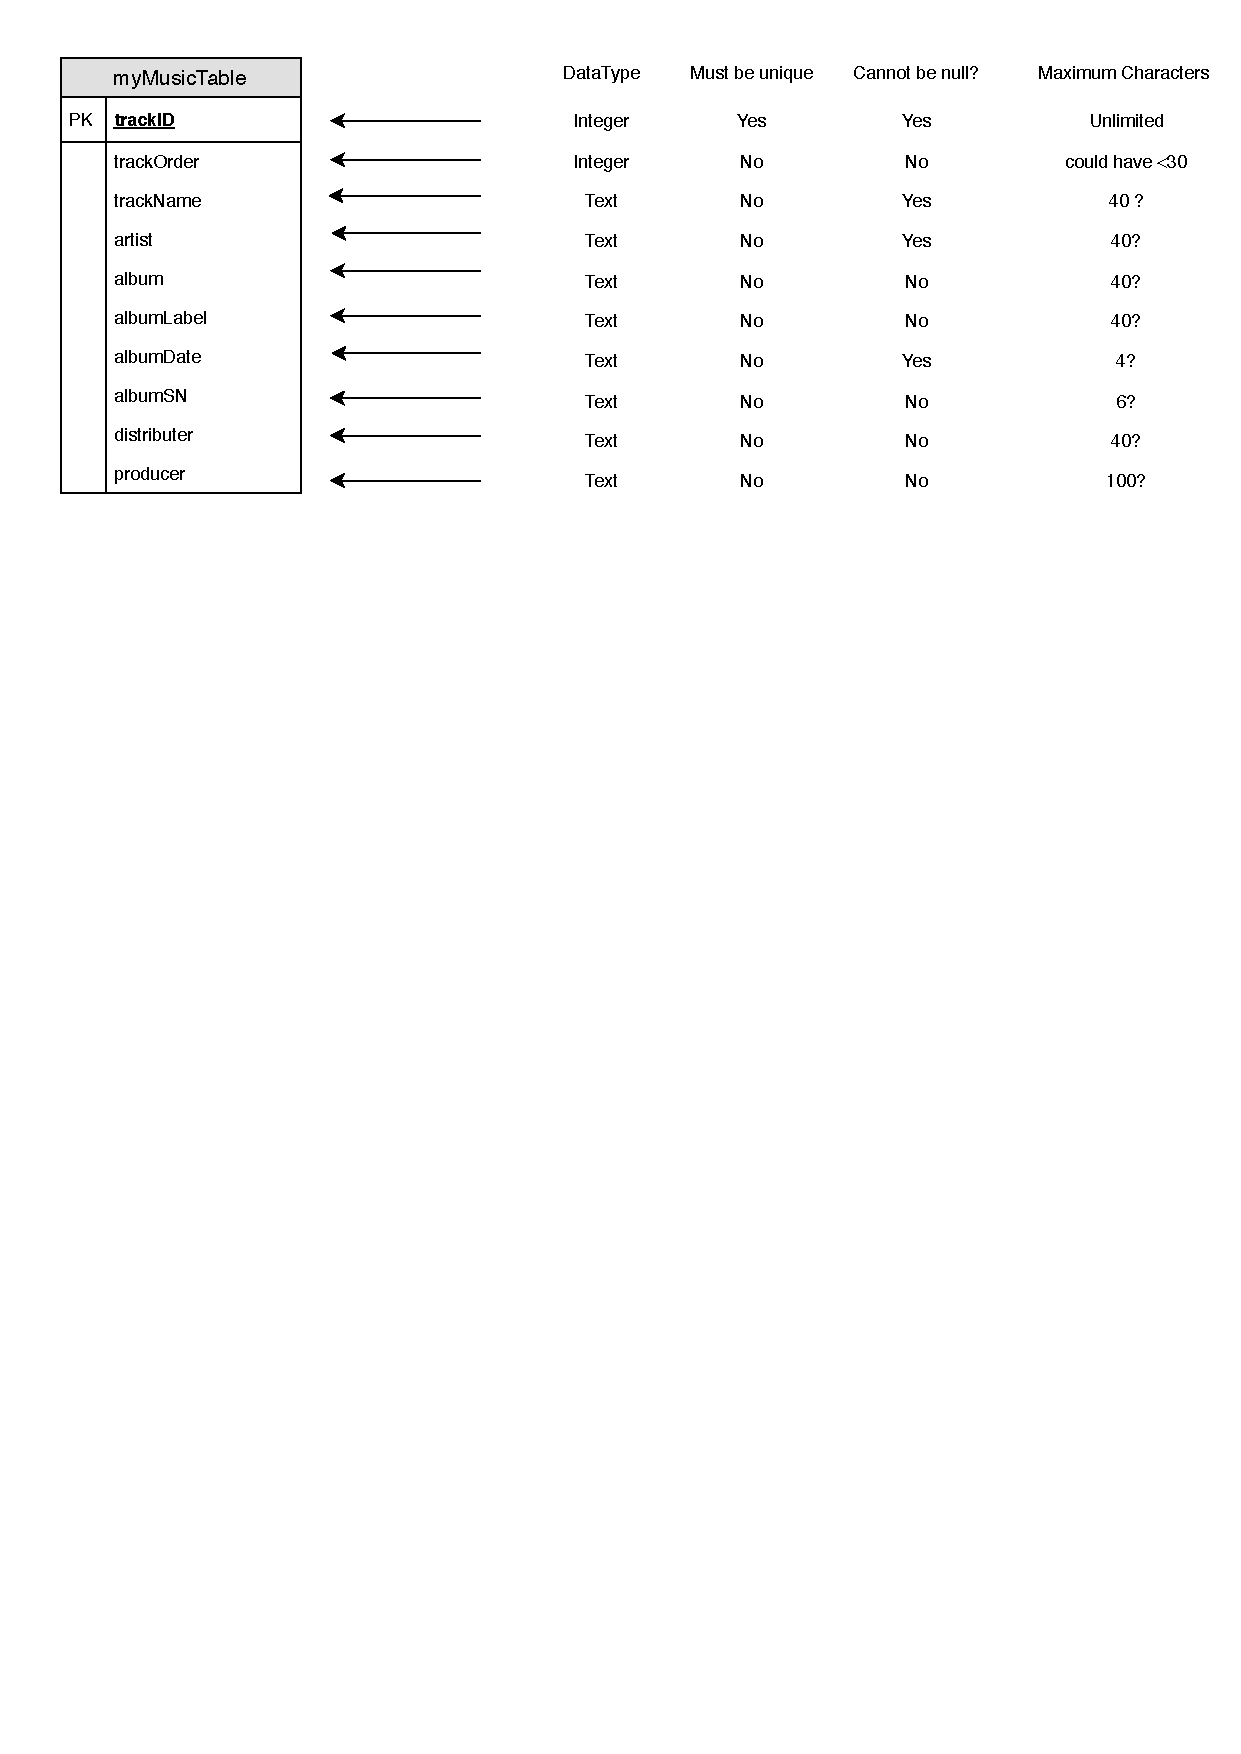
\includegraphics[width=15.5cm]{DataBaseDiagrams-SingleTable.pdf}
\end{figure}


The data types defined are very simple  in the SQLite environment.

\begin{figure}[!h]
	\centering
	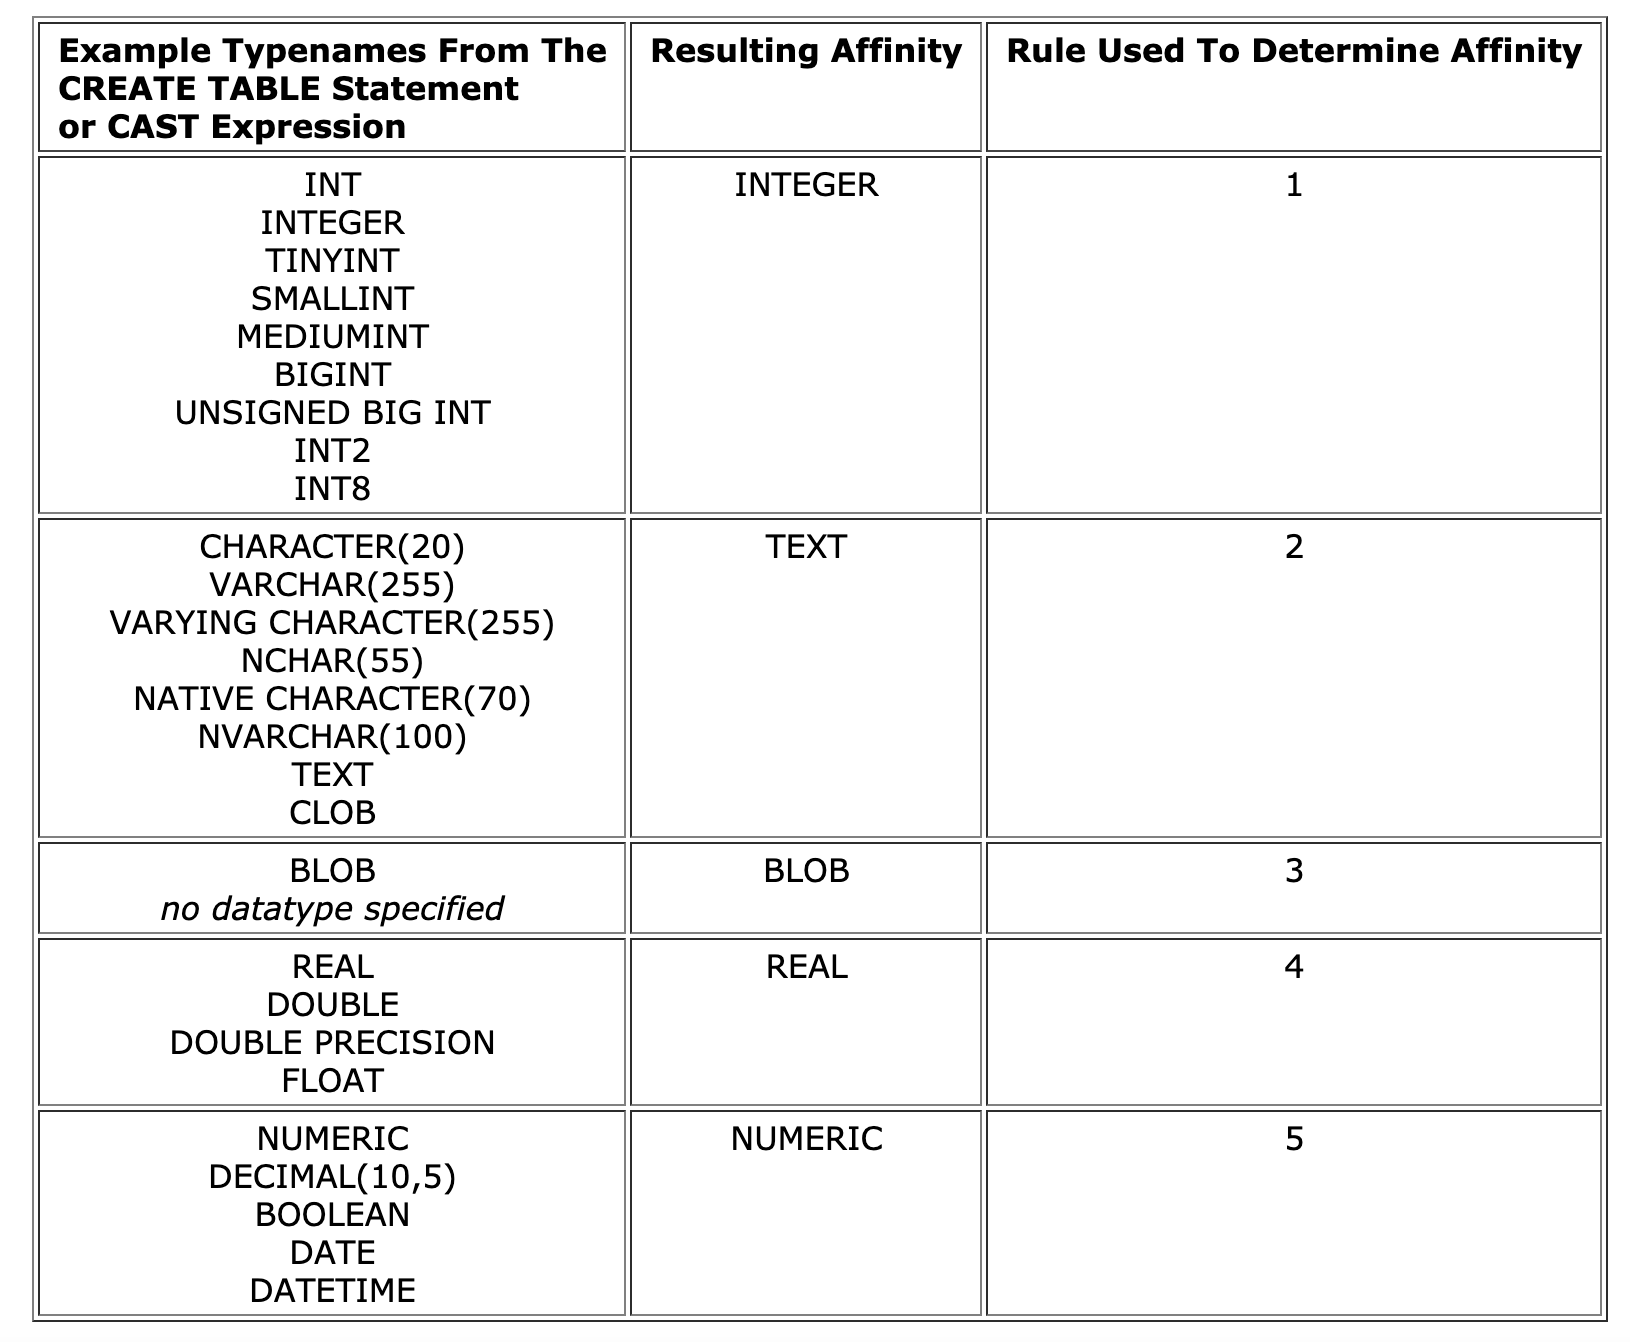
\includegraphics[width=10cm]{sqlite_affinities.png}
	\caption*{SQLite affinities}
\end{figure}

We also need to specify if the data must be unique in a particular field, and if the field can have empty cells).\\
Ideally empty cells is something we like to avoid.\\
The code for creating the table is below.\\
By defining a field as the primary key, this also will be understood as being unique and the database will automatically generate a primary key.\\

 

%Importing code from file
\lstinputlisting[language=SQL, 
caption=create myMusicTable
]{create_myMusicTable_2020.sql}

Once this has been created we can upload a csv of the data in our spreadsheet and copy it across into the myMusicTable (see video)\\

\lstinputlisting[language=SQL, 
caption=create myMusicTable
]{insert_into_myMusicTable_2020.sql}

Ensure you delete the temporary table after you have copied the data across.
\lstinputlisting[language=SQL, 
caption=delete a table
]{drop.sql}

\subsection{Basic Queries}
At this point we have a simple database and it is worth exploring how data is read from it.\\
It is important to imagine that in any real data base, they may be many thousands or even millions of rows.\\
The idea of scrolling through the data is not an option.\\
Let's consder some things we might want to find from the data
\begin{itemize}
	\item Find all tracks
	\item Find all tracks by The Cars (Showing the producer)
	\item Find all tracks before 1986 (include band and label in the output)
	\item Find the artist called Club ``something'' and show their albums 
	\item Organise the tracks by Berlin in alphabetical order ( include label and producer ).
	\item Find all tracks produced by Georgio Moroder
	\item Find out how many different albums are in the data base.
\end{itemize}
Access https://www.w3schools.com/sql/ to reserach how to do this. 
\lstinputlisting[language=SQL, 
caption=query example
]{q_set/q1.sql}
\lstinputlisting[language=SQL, 
caption=query example
]{q_set/q2.sql}
\lstinputlisting[language=SQL, 
caption=query example
]{q_set/q3.sql}
\lstinputlisting[language=SQL, 
caption=query example
]{q_set/q4.sql}
\lstinputlisting[language=SQL, 
caption=query example
]{q_set/q5.sql}
\lstinputlisting[language=SQL, 
caption=query example
]{q_set/q6.sql}
\lstinputlisting[language=SQL, 
caption=query example
]{q_set/q7.sql}
\lstinputlisting[language=SQL, 
caption=query example
]{q_set/q8.sql}
\lstinputlisting[language=SQL, 
caption=query example
]{q_set/q9.sql}

\section{Designing Part 2}
Our current database has limitations and the main one is that there is a large amount of repetition.\\
Apart from using up a lot of space, this is also problematic if we needed to alter the data (as each repeated block of data would have to be updated separately).\\
We could also consider the problems we would face if we wanted to add some further information fields about the albums (more repetition)\\\\
\textbf{Second Normal Form}
\begin{itemize}
	\item The data must be in First Normal Form
	\item The database does not have distinct tuples with the same value.
\end{itemize}
An example of a distinct tuple in our case is:  ``The Cars,Panorama,Elektra,1980,5E-514,WEA''\\
It is debatable to include the producer but we can have more than one producer per album.\\

To solve this probem we move the albums to a separate table.\\
Our data base design now looks like the two boxes and the connector in the picture below.

\begin{figure}[!h]
	\centering
	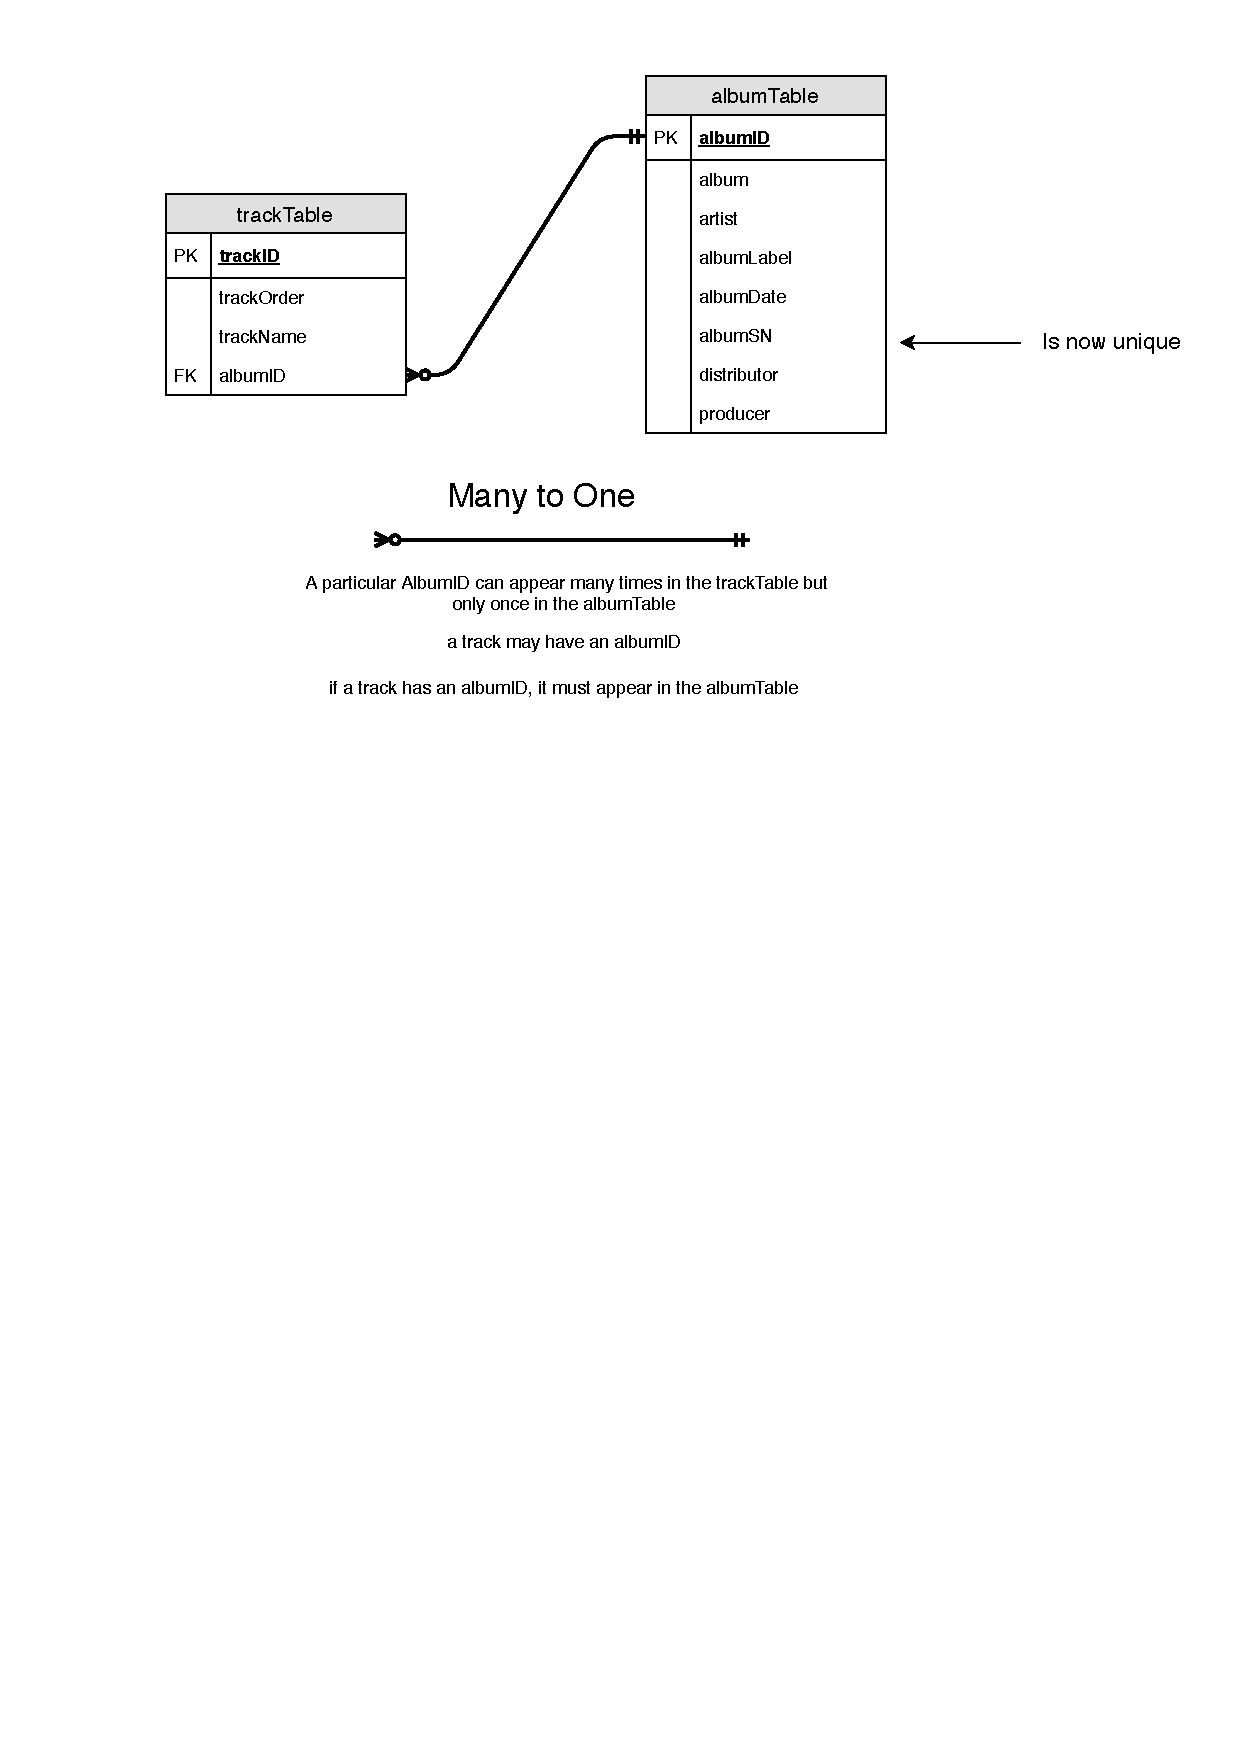
\includegraphics[width=15.5cm]{DataBaseDiagrams-MusicTable_2Tables_2020.pdf}
\end{figure}

In order to relate the trackTable with the album table, we need to use a unique key from one table and use it in the other.\\
It is logical use the primary key from one table and apply it as a \textbf{foreign key} in the other.\\
Data bases that relate tables in this way are called \textbf{relational databases}\\
To make the relationship clear we use identical field names in both.\\
How the foreign key and the primary key relate to each other is communicated using "Entity Relationship Connectors"\\
This can be discussed further in class but the key point at this stage is to either use connectors from the first group or the second group.\\

\begin{figure}[!h]
	\centering
	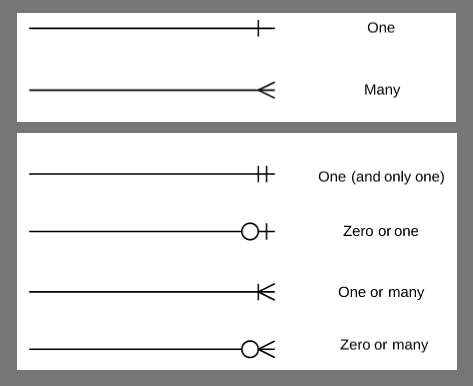
\includegraphics[width=8cm]{ERD_better_opt.png}
	\caption*{Entity Relationship Connectors}
\end{figure}

To build our database the best way is to upload the album data first and then write in the foreign keys before uploading the tracks data (see video ).\\

If we were using forms to enter the data, we would probably set up the album information and then, when entering tracks we could access the appropriate album from a list of available albums.\\
In a database context a list of already available items is called a ``lookup''.\\
\begin{figure}[!h]
	\centering
	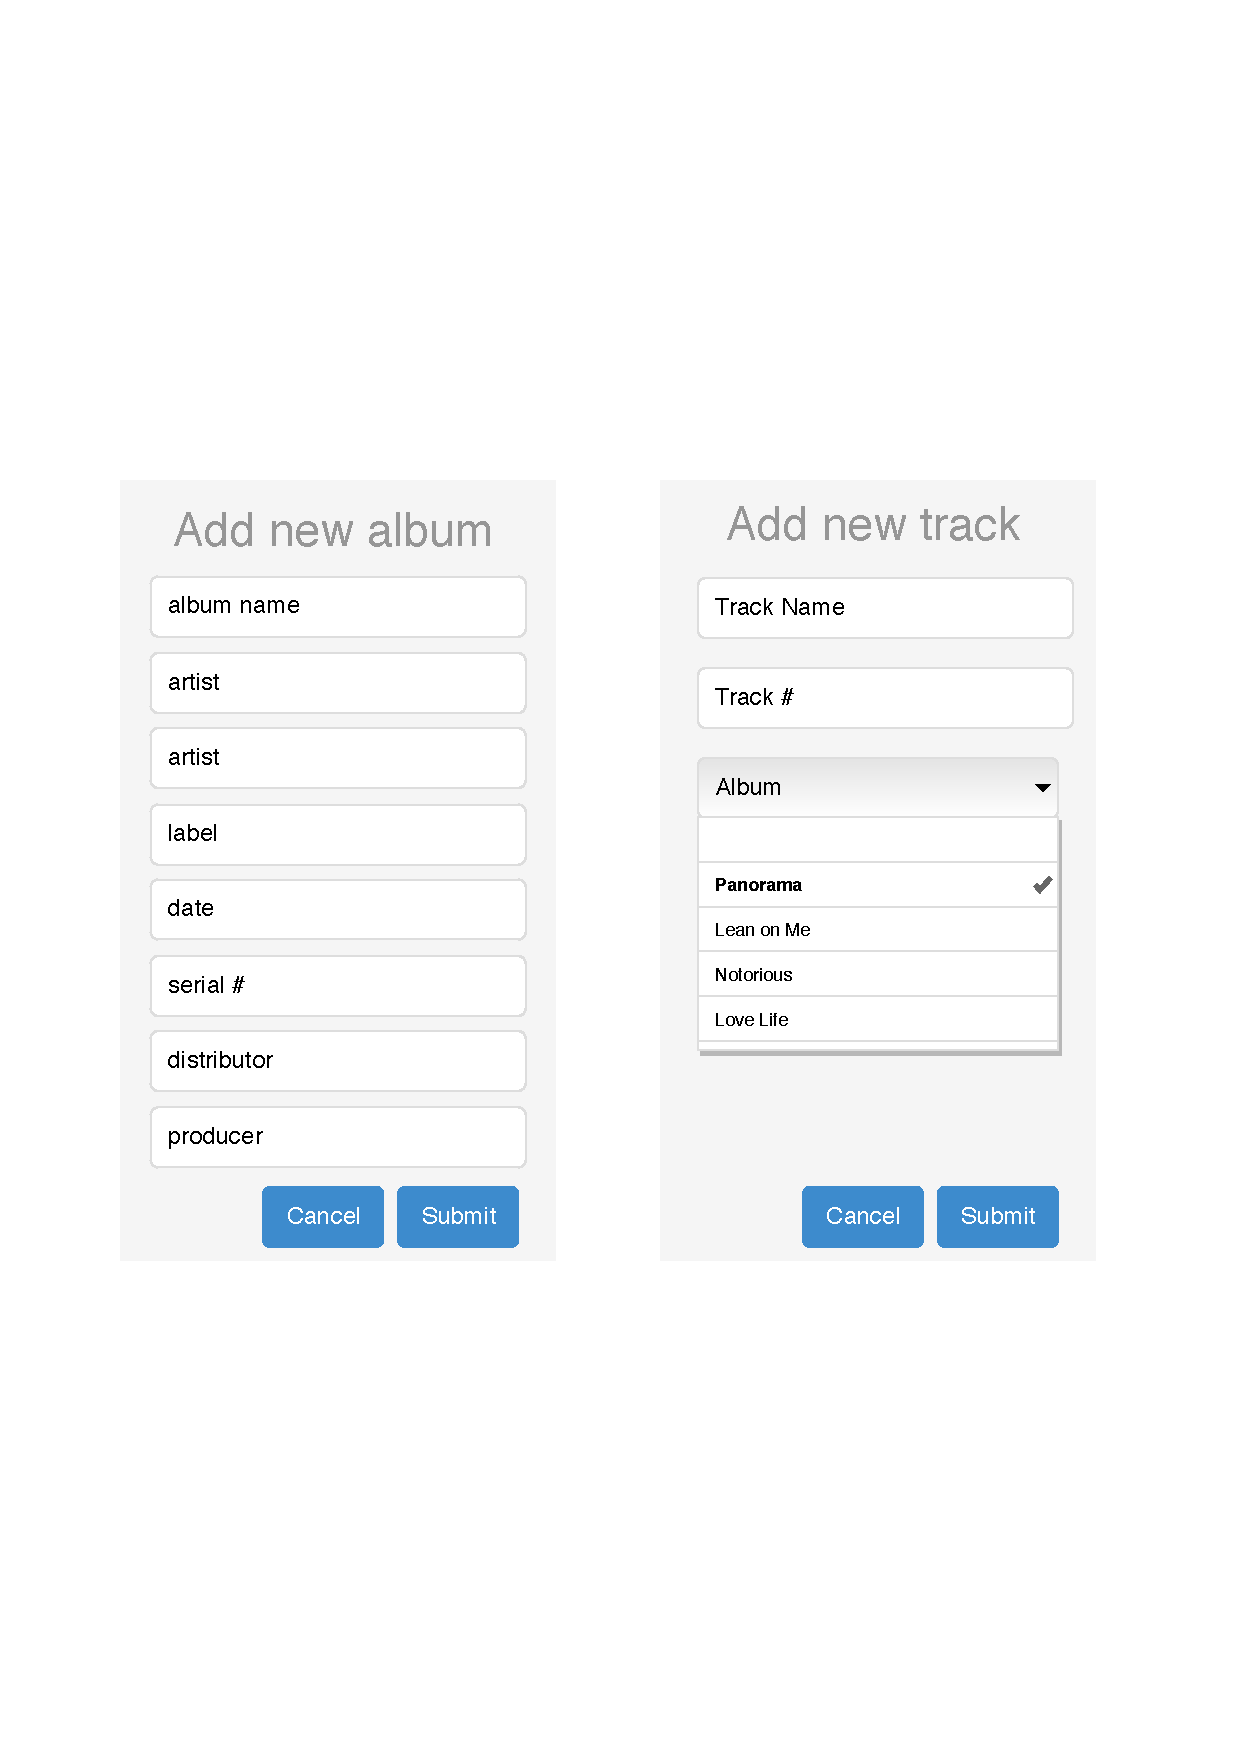
\includegraphics[width=9cm]{DataBaseDiagrams-MiniForms.pdf}
\end{figure}
\newpage
\subsection{Basic set-up code for the new database}
\lstinputlisting[language=SQL, 
caption=create album table
]{createalbum2.sql}

Upload the csv data and copy across

\lstinputlisting[language=SQL, 
caption=copy data from temp
]{insertintoalbum2.sql}

\lstinputlisting[language=SQL, 
caption= delete temporary table
]{drop2.sql}

\lstinputlisting[language=SQL, 
caption=create track table
]{createtrack2.sql}

Upload the csv data and copy across

\lstinputlisting[language=SQL, 
caption=copy data from temp
]{insertintotrack2.sql}

\lstinputlisting[language=SQL, 
caption=delete temporary table
]{drop2.sql}


\subsection{Joining}
In order to execute queries across both tables, we need to perfom a \textbf{join}.
If we wish to show all songs on the album ``Love Life''.\\\\
We
\begin{itemize}
	\item define the fields we want to appear this time using dot syntax to identify which tables we are referring to
	\item we identify the first table we are taking from
	\item join the next table and identify the equal references (i.e primary key and foreign key)
	\item add any restrictions to the query
\end{itemize}
\lstinputlisting[language=SQL, 
caption=joining
]{joinon2.sql}
\newpage
find all owners of a Berlin album
want album name  and owner name
 \section{Designing part 3}
 \subsection{Association tables}
 Let's extend our database further.\\
 Consider we want to store information about people and which of the records they own.\\
 Let's assume we are only interested whether the person owns an album or not (not whether they have more than one copy of the album).\\
 We also assume that we are talking about physical records (discs) so they cannot own some of the tracks on an album.\\
 We will have Amy, Belinda, Carman, Delia, Esther and Francesca who live in Northland, Karori, Wadestown, Northland, Thorndon and Karori respectively.
 \begin{itemize}
 	\item Amy owns Panorama and Lean On Me
 	\item Belinda owns no albums
 	\item Carman owns Notorious and Love Life
 	\item Delia owns Lean On Me and Love Life
 	\item Esther owns Panorama, Lean On Me, Notorious and Love Life
 \end{itemize}
This information needs to be stored in the data base.\\
Let's look at what happens in the database if we store this information in the albums table.

\begin{figure}[!h]
	\centering
	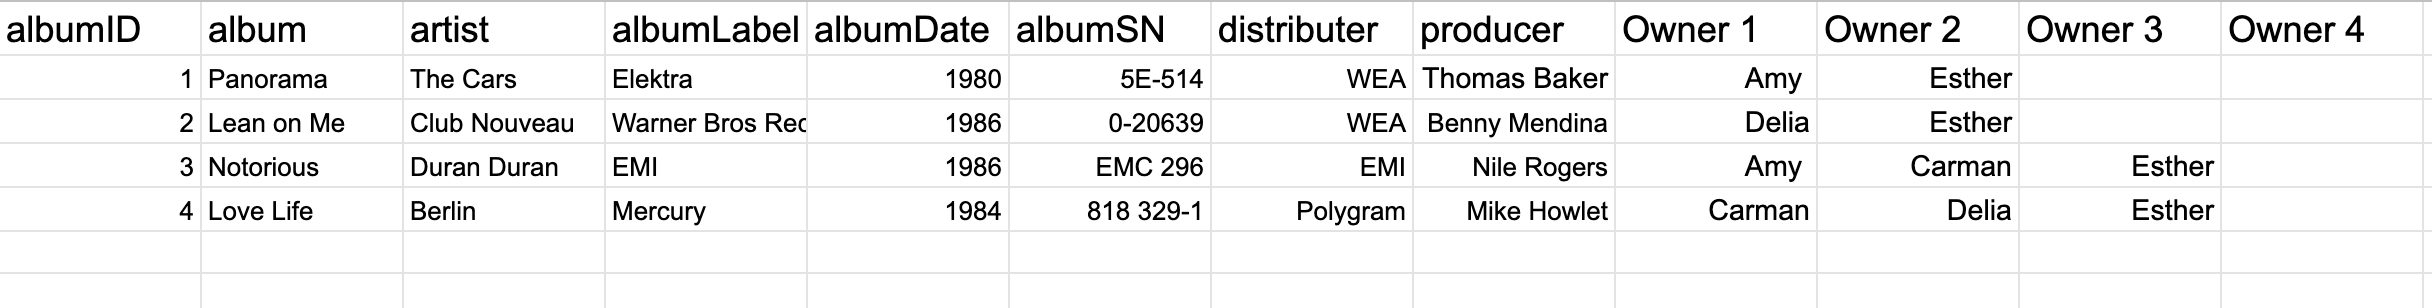
\includegraphics[width=18cm]{Owners_In_Album.png}
	\caption*{albumTable with owners added at the end}
\end{figure}

This is clearly very problematic,
\begin{itemize}
	\item Many empty cells.
	\item We have no idea what the maximum number of owners could be in the future.
	\item It makes things even more difficult if we want to include further information about the owners.
	\item There is a contradiction of Entities (Albums are one Entity and People are another).
	\item If our database is well designed we should be able to add new entities without interfering with those that are already included.
\end{itemize}
What we have have in this case is \textbf{repeating groups} (of owners) and although we have not seen it until now this is always the first problem that is dealt with when normalising a database. \\\\
It is also interesting to note that we have a many - to - many relationship between albums and owners.\\
Many albums can be owned by a particular owner and Many owners can have the same album.\\
(many albums can be owned by many owners and many owners can have many albums)\\\\

To resolve this design problem we clearly need a table for the owners (a distinct entity).\\
But we also need another table to manage the \textbf{association} between the Albums and the Owners.\\
Unsurprisingly this is called an \textbf{association table}.\\

\begin{figure}[!h]
	\centering
	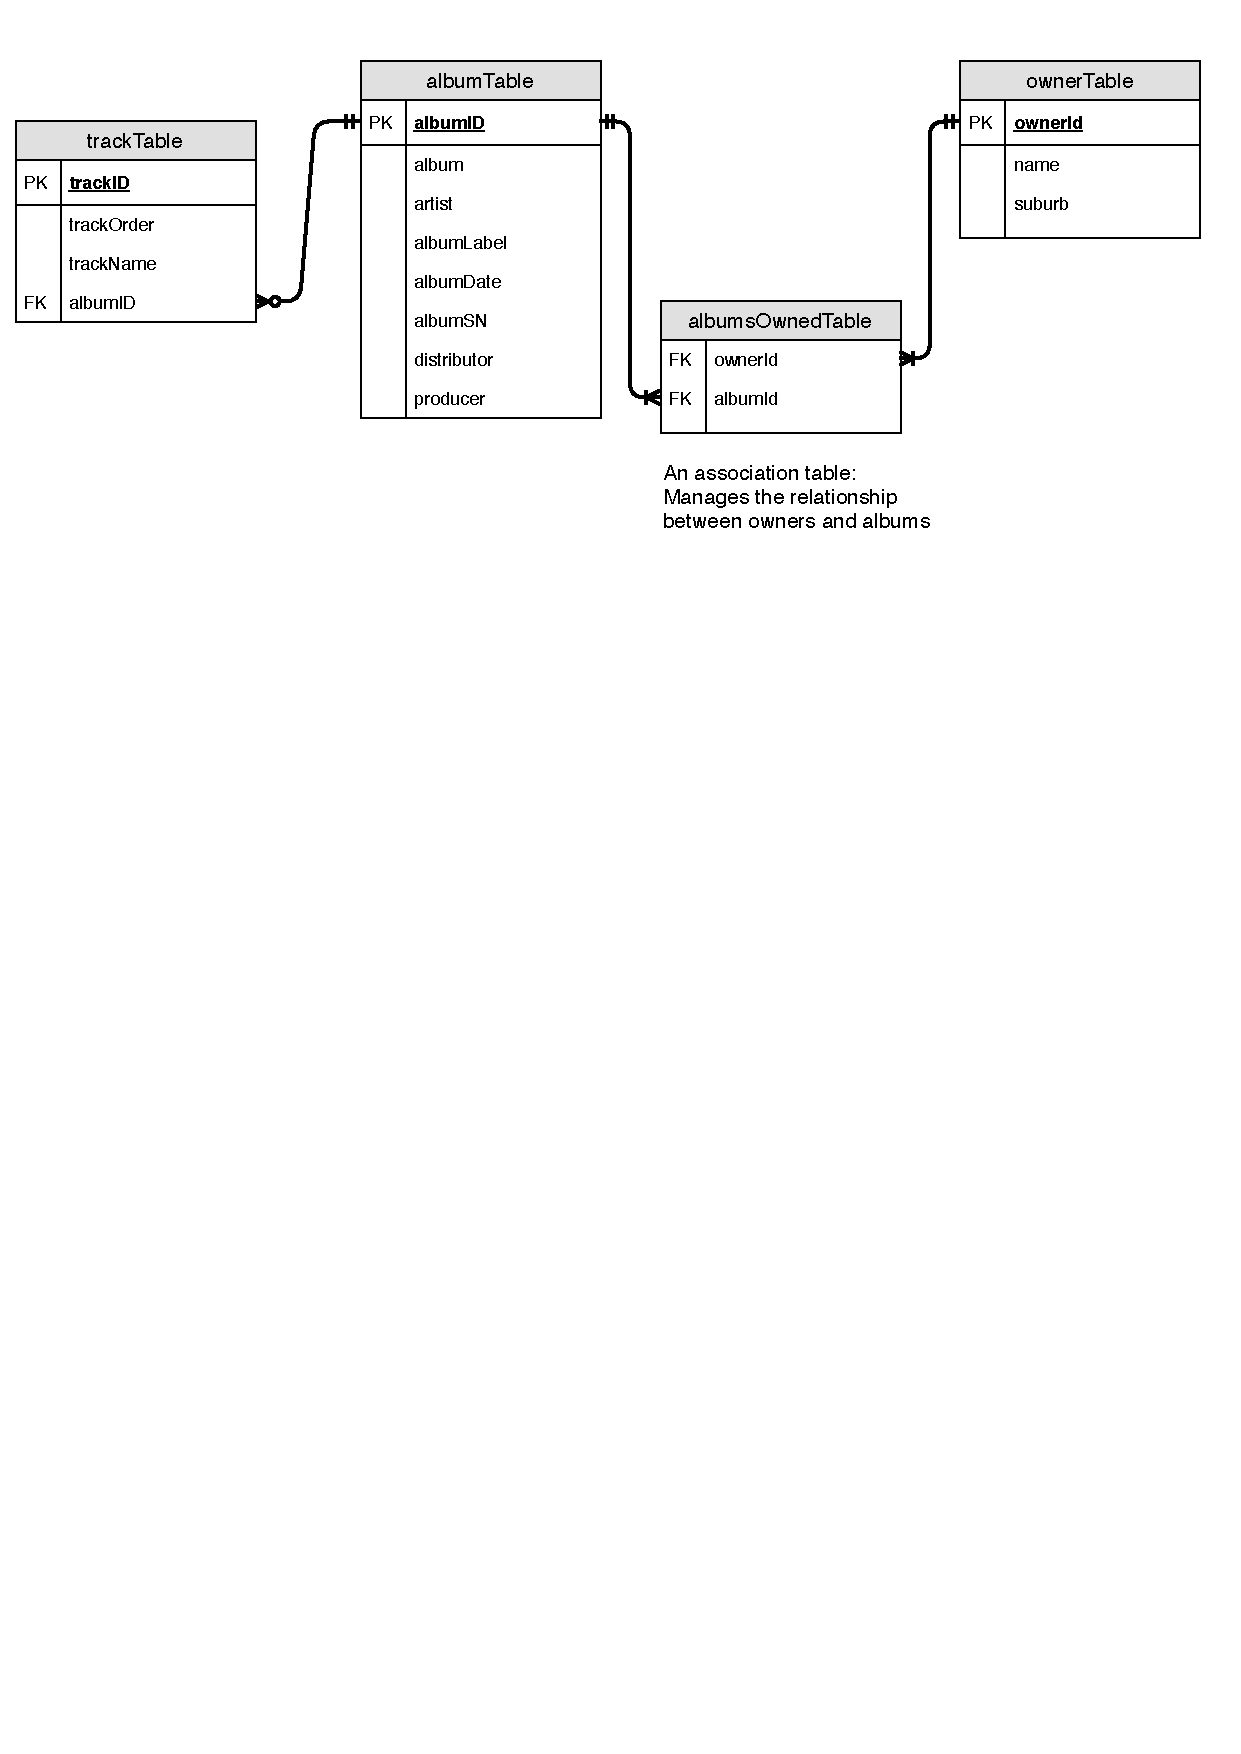
\includegraphics[width=18cm]{DataBaseDiagrams-AssociationMusic.pdf}
	\caption*{music database with association table}
\end{figure}

Assuming each person can only own a particular album or not (we are not interested in multiple copies), We could consider the \textbf{combination} of ownerId and albumId as the primary key.\\
So the primary key is a combination of two foreign keys.\\
You can see in one of the examples below how this is implemented.\\\\
 \subsection{Joining}
Joining now becomes more complicated, but the basic rules of joining are
\begin{itemize}
	\item you can have as many joins as you need
	\item start at one ``end'' and join your way to the other ``end''.
\end{itemize}

Below is some code examples for implementing the two new tables.\\

\lstinputlisting[language=SQL, 
caption=creating owner table
]{q_set2/q1.sql}
\lstinputlisting[language=SQL, 
caption=copying across temporary table
]{q_set2/q2.sql}
\lstinputlisting[language=SQL, 
caption=creating table of albums owned (note primary key definition)
]{q_set2/q3.sql}
\lstinputlisting[language=SQL, 
caption=copying across temporary table
]{q_set2/q4.sql}
\lstinputlisting[language=SQL, 
caption=trying to add a value pair that is already present in the albumsOwnedTable\\ (this should produce a uniqueness error)
]{q_set2/q5.sql}

\lstinputlisting[language=SQL, 
caption=all albums and owners
]{q_set2/q7.sql}
\lstinputlisting[language=SQL, 
caption=all tracks and owners
]{q_set2/q8.sql}
\lstinputlisting[language=SQL, 
caption=counting how many albums each person owns
]{q_set2/q9.sql}
\lstinputlisting[language=SQL, 
caption=let's give Francesca a record.
]{q_set2/adding_for_francesca.sql}
\lstinputlisting[language=SQL, 
caption=delete Amy from the system 
(so all foreign key references to Amy and then Amy herself).
]{q_set2/deleting_all_records_for_Amy.sql}
\lstinputlisting[language=SQL, 
caption=re-entering Amy into the system (she will now have a new primary key).
]{q_set2/re-Inserting_amy_and_two_albums.sql}



 
 
 
 
 
\newpage

\begin{figure}[!h]
	\centering
	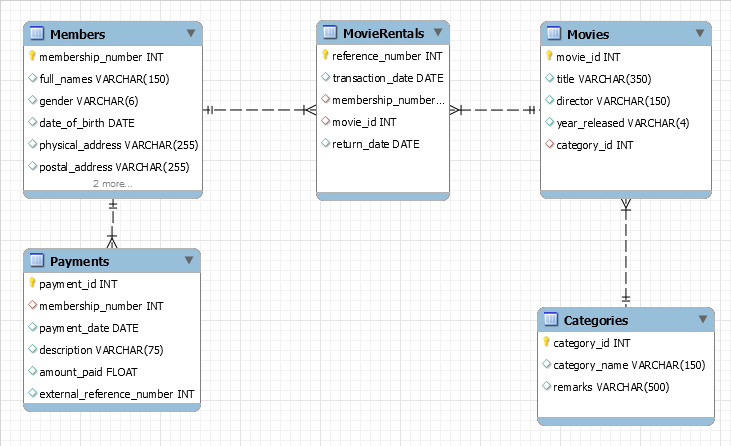
\includegraphics[width=16cm]{myflix_erd.png}
	\caption*{Movie Rentals Entity Relationship Diagram}
\end{figure}

\begin{figure}[!h]
	\centering
	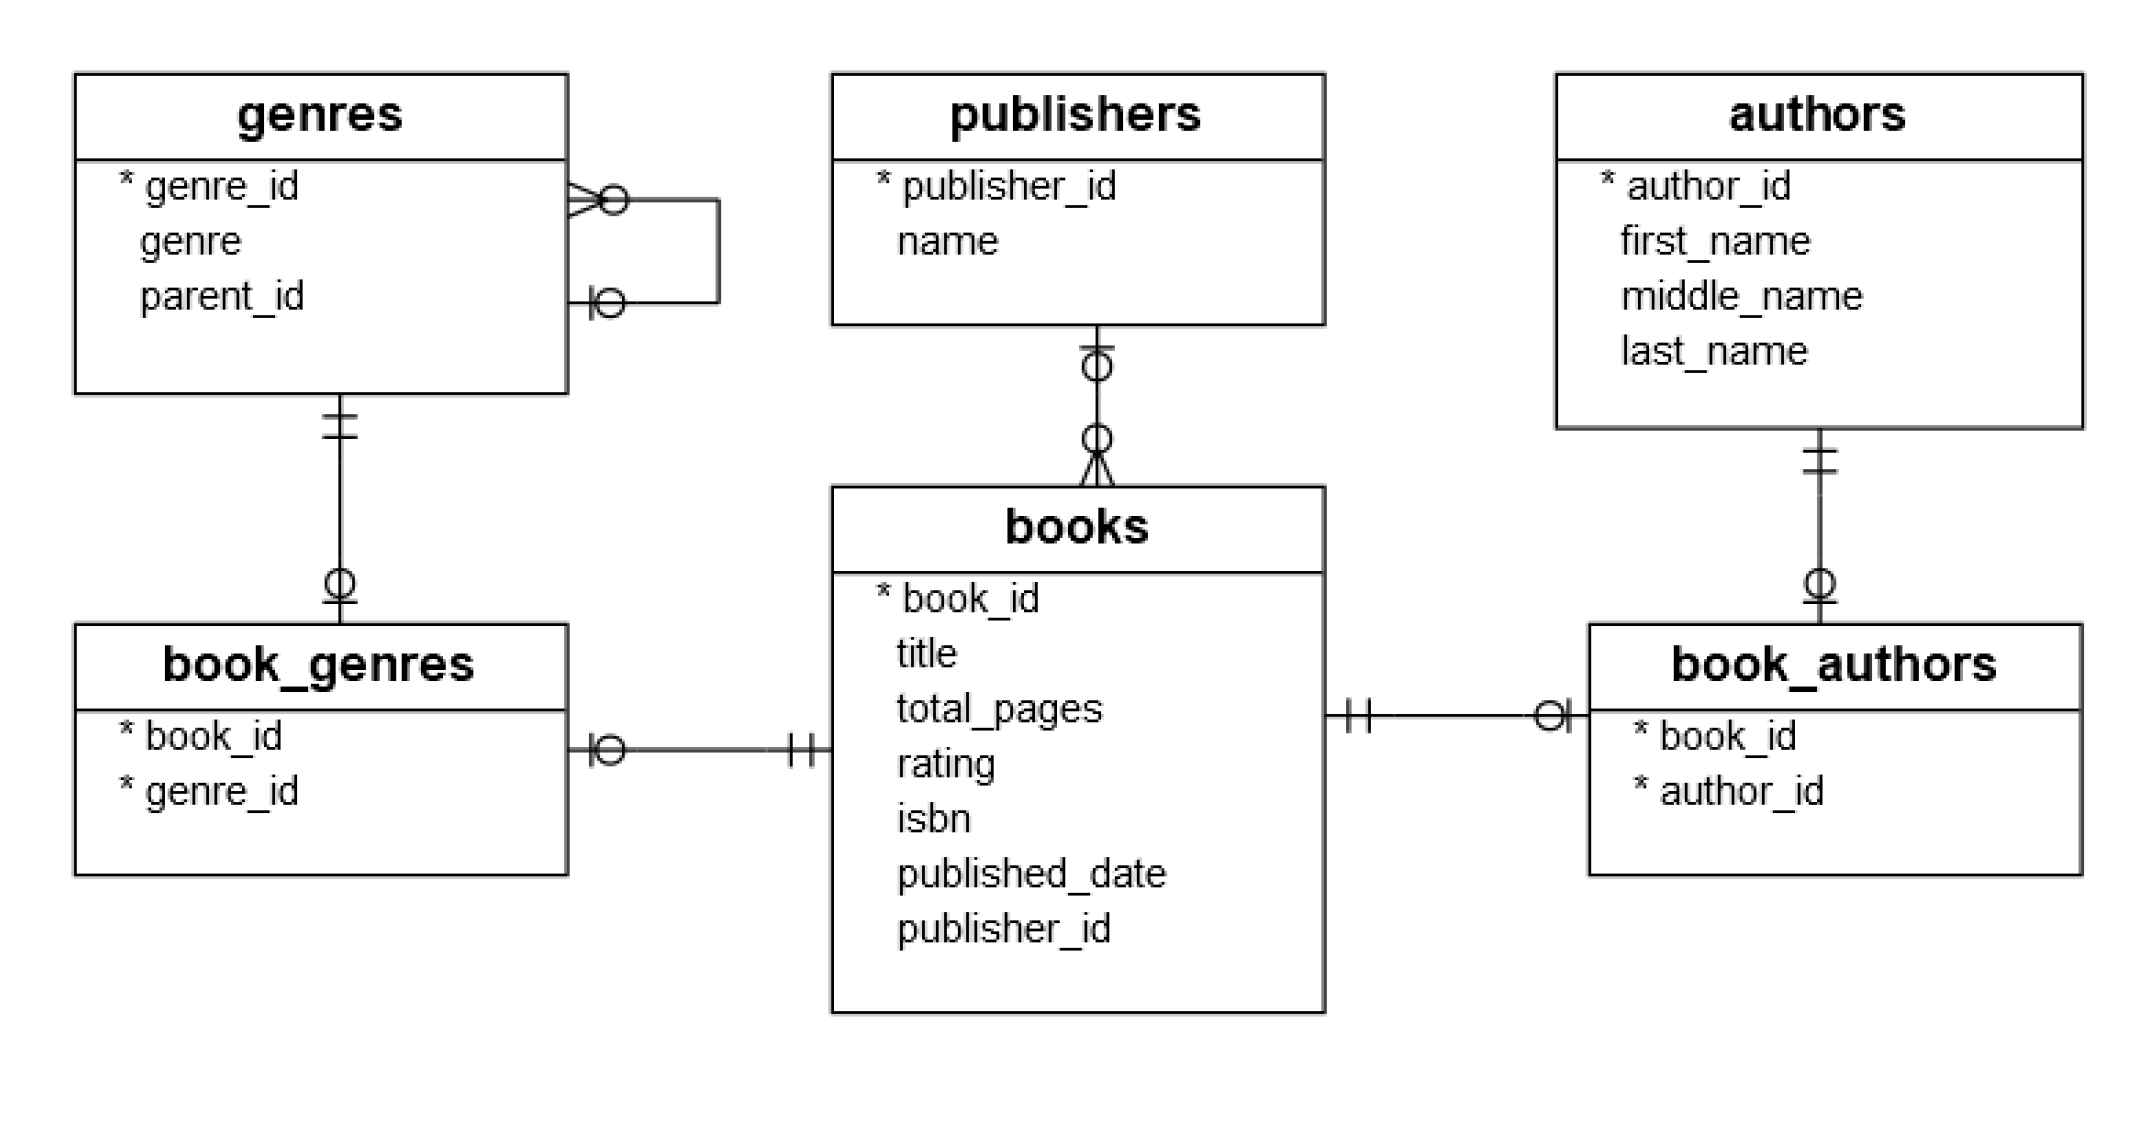
\includegraphics[width=16cm]{book_plan.png}
	\caption*{Book DataBase Entity Relationship Diagram}
\end{figure}






\end{document}